\section{Graph classes}
In this paper, we are mostly interested in classes of finite graphs\footnote{A class is a notion similar to that of a set, but classes can be larger than sets -- i.e., all finite graphs do not form a set, but form a class. For the purpose of this paper, we could identify a class of graphs $\Cc$ with a property $P$ of graphs expressed in mathematical language (such as e.g. planarity), and instead of writing $G\in\Cc$,
we would say that $G$ has  property $P$.
We could also avoid using classes and talk only about sets, but this would require restricting the vertex-sets of the considered graphs to subsets of some fixed set, e.g. $\N$. All the results in this paper would remain valid, but in the proofs we would have to pay a bit more attention to make sure that all constructed graphs only have natural numbers as vertices.}. 
By $\Gr$ we denote the class of all finite graphs,
and by $\Cc\subset \Gr$ we denote a class of finite graphs. Throughout this paper, unless stated otherwise, when speaking of graphs, we assume them to be finite.
Moreover, we  identify two graphs if they are isomorphic. 
In particular, we assume that every graph class $\Cc$ is closed under isomorphism, i.e., if $G,H$ are isomorphic graphs and $G\in\Cc$, then also $H\in \Cc$. 
By $\cliques$ we denote the class of all cliques.

\begin{example}\label{ex:classes}
Below are several classes of graphs which are of interest 
in this paper.
\begin{enumerate}
	\item The class $\cal P$ of all \emph{planar} graphs. A  graph is planar if and only if neither the clique $K_5$ nor the complete bipartite graph $K_{3,3}$ is its minor. Incidentally, planar graphs are exactly those which do not contain $K_5$ nor $K_{3,3}$ as a \emph{topological} minor.

	\item More generally, for any graph $H$, we may consider the class $\Mm_H$ of all graphs $G$ which \emph{exclude $H$ as a minor}, i.e., graphs $G$ such that $H$ is not a minor of $H$. If $H$ is a graph with at least one edge and $\Cc$ is a class of graphs contained in $\Mm_H$, then we say that the class $\Cc$
	\emph{excludes} a minor.
	Similarly we define the class $\Tt_H$ of all graphs $G$ which \emph{exclude $H$ as a topological minor},
	and say that a class $\Cc$ excludes a topological minor if it is contained in $\Tt_H$, for some graph $H$ with at least one edge. Note that every class which excludes a  minor in particular excludes a topological minor.
	
	
	\item The class ${\cal D}_d$ of all graphs in which all vertices have degrees bounded by $d$.
	This class does not exclude any graph $H$ as a minor. Indeed, for any fixed $n$, the clique $K_n$
	is a minor of a $3$-regular graph $G$ obtained by replacing every vertex $i\in\set{1,\ldots,n}$ in $K_n$ by a path $P^i$ of length $n-1$,
and replacing the $n-1$ edges leaving from $i$	in $K_n$ by $n-1$ edges leaving from consecutive vertices of $P^i$. However, ${\cal D}_d$ is a class which excludes a topological minor, e.g., it excludes $K_{d+1}$ as a topological minor.
	
	\item The class of all graphs of treewidth bounded by a fixed number $d$. We omit the definition of treewidth here, see e.g.~\cite{??}. The class of all graphs of treewidth at most $d$ excludes a minor. More precisely, there is a function $f:\N\to\N$ such that 
	every graph of treewidth $d$ excludes the $k\times k$ grid as a minor where $k=f(d)$.


\end{enumerate}
\end{example}
%
% \subsection{Graph parameters}
% A \emph{graph parameter} is a function $f:\Gr\to \Rbar$, where $\Rbar=\R\cup\set{-\infty,+\infty}$, which is invariant under isomorphism, i.e., $f(G)=f(H)$ for isomorphic graphs $G,H$.
% For example, denote by $\omega(G)$ the maximal number of vertices of a clique $H$ contained (as a subgraph) in $G$.
% Then $\omega$ is a graph parameter.
%
% We consider several graph parameters.
% \begin{itemize}
%   \item For $d\in\N$, let $\omega_d(G)$ denote the maximal number $n$ such that $K_n$ is a minor at depth $d$ of $G$.
%
%   \item Similarly, for  $d\in\N$, let $\tilde\omega_d(G)$ denote the maximal number $n$ such that $K_n$ is a topological minor at depth $d$ of $G$.
%
% \item For $d\in\N$, let $\nabla_d(G)$ denote the maximum
% of $\frac{|E(H)|}{|V(H)|}$, ranging over all graphs $H$ such that $H$ is a minor at depth $d$
% of $G$.
%
% \item For $d\in\N$, let $\nabla_d(G)$ denote the maximum
% of $\frac{|E(H)|}{|V(H)|}$, ranging over all graphs $H$ such that $H$ is a topological minor at depth $d$
% of $G$.
% \end{itemize}
%
%
% Theorem~\ref{thm:nowhere-dense} expresses the fact that in some sense, the  the above graph parameters are all equivalent. To make this equivalence precise, we make the following definitions.
%
% A \emph{graph parameter sequence} is a sequence $f_1,f_2,\ldots$ of graph parameters. Such a sequence will be denoted $f\seq$. If $f\seq$ and $g\seq$ are two graph parameter sequences, then we write that $f\seq\preceq g\seq$
% if there exist increasing functions $s,t:\N\to\N$
% such that $f_n(G)\le s(g_{t(n)}(G))x$, for every graph $G$.
% If $f\seq\preceq g\seq$ and $g\seq\preceq g\seq$, then we write $f\seq \simeq g\seq$.
%
% \begin{theorem}\label{thm:nowhere-dense1}
%   The graph parameter sequences $\omega\seq,\tilde\omega\seq,\nabla\seq,\tilde\nabla\seq$
%   are all equivalent with respect to $\simeq$.
% \end{theorem}

\paragraph{Class operations}
We introduce some convenient notation for applying operations to graph classes.
If $\Phi$  is an interpretation and $\Cc$ is a class of finite graphs, then by $\Phi(\Cc)$ we denote the class $\setof{\Phi(G)}{G\in \Cc}$.

Let $R$ be a binary relation on graphs, i.e., a class $R\subset \Gr\times \Gr$.
By $R(\Cc)$ we denote the class of all graphs $H$
such that the relation $R$ holds of $H$ and $G$, for some graph $G\in \Cc$, i.e.,
$$R(\Cc)=\setof{H\in \Gr}{\exists G\in \Cc. (H,G)\in R}.$$
For example, define the relation $\subgraph$
so that $(H,G)\in\subgraph$ if and only if $H$
is isomorphic to a subgraph of $G$. Then $\subgraph(\Cc)$
is the class of all subgraphs of graphs from $\Cc$.
Similarly, $\minor{}(\Cc)$ denotes the class of all graphs which are a minor of a graph in $\Cc$,
$\minor d (\Cc)$ denotes the class of all graphs which are a minor at depth $d$ of some graph $G\in\Cc$,
and $\tminor d (\Cc)$ denotes the class of all graphs which 
are a topological minor at depth $d$ of some graph $G\in 
\Cc$. Incidentally, $\minor 0 (\Cc)=\tminor 0 
(\Cc)=\subgraph(\Cc)$. Consistently with the above 
convention, $\indsub(\Cc)$ denotes the class of all induced 
subgraphs of graphs in $\Cc$.
A class $\Cc$ is \emph{closed under subgraphs} if $\Cc=\subgraph(\Cc)$, is \emph{closed under induced subgraphs} if $\Cc=\indsub(\Cc)$, and is \emph{minor-closed}
if $\Cc=\minor{}(\Cc)$.
By  $\subdiv k\Cc$ (respectively, $\msubdiv k \Cc$) we denote the class of graphs $H$
such that $H$ is the (maximal) $k$-subdivision of some graph in $\Cc$.




\subsection{Nowhere-denseness}
% For a class of graphs $\Cc$ and a number $d$,
% let $\minors d\Cc$ denote the class
% of all graphs which are a minor at depth $d$
% of some graph $G\in\Cc$. Similarly, by $\tminors d \Cc$ we denote the class of all graphs which are a topological minor at depth $d$ of some graph $G\in\Cc$.
%

The main result presented in this section is the following theorem.
\begin{theorem}\label{thm:nowhere-dense}
	Let $\Cc$ be a class of graphs. 
	The following conditions are equivalent.
	\begin{enumerate}
		\item\label{it:clique-minor}  $\minors d\Cc=\Gr$ for some $d\in\N$.
		In other words, 
		there is a number $d\in\N$ such that 
		every graph $H$ is a minor at depth $d$ 
		of some graph $G\in\Cc$.
		
		\item\label{it:clique-topminor}  $\tminors d\Cc=\Gr$ for some $d\in\N$. %In other words, there is a number $d\in\N$ such that 
%		every graph $H$ is a topological minor at depth $d$ 
%		of some graph $G\in\Cc$.
		
		\item\label{it:dense-minor} There is a number $d\in \N$ and a number 
		   $\eps>0$ such that 
		there are arbitrarily large graphs $H\in\minors d\Cc$ with $\frac{|E(H)|}{|V(H)|}> |V(H)|^{1-\eps}$.
		
		\item\label{it:dense-topminor} There is a number $d\in \N$ and a number 
		   $\eps>0$ such that 
		there are arbitrarily large graphs $H\in\tminors d\Cc$ with $\frac{|E(H)|}{|V(H)|}> |V(H)|^{1-\eps}$.
	\end{enumerate}
\end{theorem}


We say that a class $\Cc$ is \emph{somewhere dense}
if it satisfies one of the equivalent conditions above;
otherwise it is called \emph{nowhere dense}.
In particular, $\Cc$ is nowhere dense if and only if it satisfies one of the following, equivalent conditions.

\begin{align}
  \label{char:nd}\tag{ND1}
\begin{minipage}[c]{0.8\textwidth}\it\noindent For every $d\in \N$ there is a graph $H$ 
	such that $\Cc$ excludes $H$ as a minor at depth $d$.\medskip\end{minipage}
  \\
  \label{char:nd-top}\tag{ND2}
  \begin{minipage}[c]{0.8\textwidth}\it\noindent For every $d\in \N$ there is a graph $H$
  	such that $\Cc$ excludes $H$ as a topological minor at depth~$d$.\medskip\end{minipage}
    \\        
  \label{char:nd-dens}\tag{ND3}
  \begin{minipage}[c]{0.8\textwidth}\it\noindent For every $d\in\N$ and every $\eps>0$, if $H\in\minors d\Cc$ is sufficiently large, then $\frac{|E(H)|}{|V(H)|}<|V(H)|^\eps$.\medskip\end{minipage}
  \\
  \label{char:nd-dens-top}\tag{ND4}
  \begin{minipage}[c]{0.8\textwidth}\it\noindent For every $d\in\N$ and every $\eps>0$, if $H\in\tminors d\Cc$ is sufficiently large, then $\frac{|E(H)|}{|V(H)|}<|V(H)|^\eps$.\medskip\end{minipage}
\end{align}


\begin{example}
	The class $\Gr$ of all graphs is somewhere dense,
	so is the class $\cliques$ of all cliques,
  as well as the class $\msubdiv k \cliques$ consisting of the maximal $k$-msubdivisions of cliques, for a fixed number $k$.
  	Observe that a class $\Cc$
  is nowhere dense if and only if $\subgraph(\Cc)$ is nowhere dense. 
  Hence, when speaking of nowhere dense classes,
  it is reasonable to assume that the class is closed under 
  taking subgraphs. Also, a class $\Cc$ is somewhere dense if and only if there is a number $d\in\N$
  such that $\cliques\subset\minors d \Cc$, if and only if there is a number $d'\in\N$
  such that  $\cliques\subset\tminors {d'} \Cc$.
  \end{example}
  \begin{example}
		We verify that all classes listed in Example~\ref{ex:classes} are nowhere dense.
	\begin{itemize}
		\item For the class of planar graphs $\cal P$, we use the characterization~\eqref{char:nd}: the graph $K_5$ is not a minor at any depth of any planar graph. We could also use the characterization~\eqref{char:nd-dens}. Indeed, a minor of a planar graph is planar, and it is well known that $\frac{|E(H)|}{|V(H)|}<3$
		for all planar graphs, as a consequence of Euler's formula\footnote{Euler's formula says that 
		for every planar embedding (see Footnote~\ref{ft:planar} on page~\pageref{ft:planar}) $f$ of $G$ in $\R^2$, the number of \emph{faces}, i.e., connected components of $\R^2-\bigcup_{e\in E(G)}f(e)$ satisfies $|\textit{vertices}|-|\textit{edges}|+|\textit{faces}|=2$. Moreover,  each face touches at least $3$ edges, and each edge touches at most two faces, yielding $2|\textit{edges}|\ge 3|\textit{faces}|$. Combining the two gives $\frac{|\textit{edges}|}{|\textit{faces}|}< 3$.}.
		
		\item More generally, if a class $\Cc$ excludes $H$ as a minor, then for every $d\in \N$ the graph $H$
		is not a minor at depth $d$ of any graph $G\in\Cc$. Hence, every class excluding a minor is nowhere dense, using~\eqref{char:nd}. By a similar argument, and by using~\eqref{char:nd-top}, every class excluding a topological minor is nowhere dense.
		
		\item In particular, for every fixed $k\in \N$, the class $\Dd_k$ of graphs whose vertices have degrees at most $k$ is nowhere dense, as it excludes a topological minor. As an illustration, we check that $\Dd_k$  satisfies the  condition~\eqref{char:nd-dens}.
	First observe that if $H$ is a minor at depth $d$ of a graph $G\in\Dd_k$, then $H\in \Dd_l$ for $l=k^{d+1}$.  In particular, $|E(H)|\le l\cdot |V(H)|$.
	It follows that for a fixed number $d\in\N$ and $\eps>0$, if $H$ is such that $|V(H)|>k^{\frac{d+1}\eps}$, then $\frac{|E(H)|}{|V(H)|}\le l=k^{d+1}\le |V(H)|^\eps$.
This proves that $\Dd_k$ satisfies~\eqref{char:nd-dens}.
Since every topological minor at depth $d$	is in particular a minor at depth $d$, it follows that $\Dd_k$ also satisfies~\eqref{char:nd-dens-top}.
	\end{itemize}
\end{example}

\begin{example}\label{ex:ladders-dense}
  Let $\Cc$ be a class which contains arbitrarily large ladders.
  Then $\Cc$ is somewhere dense. Indeed -- a ladder $L_k$ has a quadratic number of edges:
  $${|E(L_k)|}=\frac{k(k+1)}{2}$$
  and if $\eps>0$ is fixed, then $\frac{|E(L_k)|}{|V(L_k)|}=\frac{k+1}4>(2k)^{1-\eps}$ for sufficiently large $k$.
Hence, by condition~\ref{it:dense-minor} of Theorem~\ref{thm:nowhere-dense}, $\Cc$ is somewhere dense.

In particular, by Theorem~\ref{thm:nowhere-dense},
 there is a number $d\in\N$ such that $\tminors d\Cc=\Gr$. This is not difficult to see directly, 
 for $d=1$.
Indeed, observe that a ladder $L_k$ contains an induced subgraph which is a complete bipartite graph with $\lfloor k/2\rfloor$  vertices in each part: this is the subgraph of $L_k$ induced by vertices of degree at least $\lceil k/2\rceil$. In particular, $L_k$ contains as a subgraph the maximal 1-subdivision of the clique with $\lfloor k/2\rfloor$ vertices. Hence, $\tminors 1\Cc$ contains arbitrarily large cliques, and therefore, all graphs.
\end{example}

The following lemma is a direct consequence of Lemma~\ref{lem:minor-transitivity}.
\begin{lemma}\label{lem:nd-transitivity}
	Let $\Cc$ be a class of graphs.
	If 	$\minors d\Cc$ or $\tminors d\Cc$ is a somewhere dense class,
	for some $d\in\N$, then $\Cc$ is somewhere dense, too.	
\end{lemma}

\begin{proof}[Proof sketch of Theorem~\ref{thm:nowhere-dense}]
  We only give a very rough sketch of the main ideas of the proof of the theorem. See~\ref{??} for more details.
  
  The implication~\impl{it:clique-topminor}{it:clique-minor}
  is immediate, since as observed in Example~\ref{ex:topminor-minor}, $\tminors d\Cc\subset\minors d\Cc$. The same applies to the implication~\impl{it:dense-topminor}{it:dense-minor}.
  
  The implication~\impl{it:clique-minor}{it:dense-minor}
  is immediate, since by assumption, for some $d\in\N$,
  $\cliques\subset\minors d \Cc$,
  and a large  clique $K_n$ has quadratic edge density; in particular, for any fixed $\eps>0$, if $n$ is large enough then $$\frac{|E(K_n)|}{|V(K_n)|}>|V(K_n)|^{1-\eps}.$$ 

The implication~\impl{it:clique-topminor}{it:dense-topminor}
follows exactly the same lines.

  The remaining, and more difficult implications are~\impl{it:dense-minor}{it:clique-minor},~\impl{it:dense-topminor}{it:clique-topminor},
  and~\impl{it:clique-minor}{it:clique-topminor}.

  
  
	\begin{figure}[h]
	  \centering
	    \includegraphics[scale=0.25,page=11]{pictures.pdf}
	  \caption{A model $B$ of $K_5$ in a graph $G$,
    with each $B(v)$ being a tree with root $\gamma(v)$.
    Thick lines depict paths, thin lines depict edges,
    and the blobs depict the subgraphs $B(v)$ of $G$.
	  } 
	  \label{fig:model}
	\end{figure}	 
  \paragraph{Implication~\impl{it:clique-minor}{it:clique-topminor}} 
  We first sketch the implication~\impl{it:clique-minor}{it:clique-topminor}.
  Fix $d\in\N$ such that $\cliques\subset\minors d \Cc$.
  We will show that $K_m\in\tminors {d'}\Cc$, for $d'=8d+4$.
  Choose a large number $n\in\N$,
  and consider the minor model $B$ of $K_n$ in $G$,
  for some $G\in \Cc$, witnessing the fact that $K_n\in \minors d \Cc$. In particular, for each vertex $v\in V(H)$,
  the graph $B(v)$ has radius at most $d$.
  Choose a ``central'' vertex $\gamma(v)\in B(v)$, 
  such that every vertex of $B(v)$ is at distance at most $d$ from $\gamma(v)$. By removing unnecessary edges from $B(v)$, we may assume that $B(v)$ is a tree, and we treat $\gamma(v)$ as the root of the tree. Figure~\ref{fig:model}
  illustrates the situation. The point is that to obtain a topological minor model of the clique $K_m$, we would like all the trees $B(v)$ to 
  be of a particularly simple form, namely, to be $d$-subdivisions of the star with $m-1$ arms. The rough idea is to restrict each $B(v)$ by choosing its subgraph $S(v)$ which is a subdivision of a star of high degree. This can be achieved, since $B(v)$ is a tree with many leaves (precisely $n-1$) and of low depth (at most $d$). In particular, if $n>(m-2)^d$, then the rooted tree $B(v)$ must contain a vertex $\sigma(v)$ of degree at least $m$.   
   We define $S(v)$ 
  as the subgraph of $B(v)$ consisting of $\sigma(v)$
  and $m-1$ paths leaving from $\sigma(v)$ downwards towards the leaves below $\sigma(v)$ in the tree $B(v)$ rooted at $\gamma(v)$. 
  
To exhibit a topological minor model of $K_m$ in $G$,
choose in $K_n$ a family of $m$ pairwise disjoint stars, each with $m-1$ arms
(this assumes that $n\ge m^2$). 
Let $v_i\in V(K_n)$ denote the center of the $i$th star;
if $w$ is a leaf in the $i$th star, we call the graph $B(w)$
a \emph{proxy} of $B(v_i)$ (see Figure~\ref{fig:proxies} below, where  we depict $B(v_2)$ and $B(v_3)$ and their proxies). 
\sz{Needs to be fixed: the $m-1$ proxies of $B(v_i)$ don't necessarily neighbor with the $m-1$ leaves of $S(v_i)$.
Follow~\cite{PT}.
}


	\begin{figure}[h]
	  \centering
	    \includegraphics[scale=0.32,page=12]{pictures.pdf}
	  \caption{In this picture, $m=5$, $i=3,j=2$. The proxies are the small blobs neighboring with $B(v_2)$ and $B(v_3)$.
	  } 
	  \label{fig:proxies}
	\end{figure}	

% Mark all $w_l$, as well as $v_i$ as ``used''.
Our constructed topological minor model will map vertex $i\in V(K_m)$ to $\sigma(v_i)$, and the edge $ji\in E(K_m)$ with $j<i$
to a path $M(ji)$ constructed as follows.

 Choose a labeling of the $m-1$ leaves of $S(v_i)$ which bijectively maps
each leave to a neighbor of $i$ in $K_m$, i.e. to a number $1\le j\le m$ different from $i$.
Choose an unused vertex $v_{ij}\in V(K_n)$, and mark it as ``used''.
Choose a path $\pi$
which:
\begin{itemize}
  \item  starts in $\sigma(v_i)$ and goes downwards in the tree $S(v_i)$ towards the leave $l$ of $S(v_i)$
  labeled $j$,
  
  \item then follows an edge from $l$ to some vertex $x$ in $B(w_l)$,
  
  \item then leads from vertex $x$ in $B(w_l)$ to a vertex 
  $x'$ adjacent to a vertex $x''$ in $B(v_{ij})$,
  and finally follows the edge from $x'$ to $x''$.
\end{itemize}
Similarly, choose a path $\rho$ which:
\begin{itemize}
  \item  starts in $\sigma(v_j)$ and goes downwards in the tree $S(v_j)$ towards the leave $k$ of $S(v_i)$
labeled $i$ (the leaves of $S(v_j)$ have been labeled 
at an earlier stage, since $j<i$),
  
  \item then follows an edge from $k$ to some vertex $y$ in $B(w_k)$
  
  \item then leads from vertex $y$ in $B(w_k)$  to  a vertex $y'$
  adjacent to a vertex $y''$ in $B(v_{ij})$,
  and finally follows the edge from $y'$ to $y''$.
\end{itemize}
Finally, let $\tau$ be a path from $x''$ to $y''$ in $B(v_{ij})$.
Note that the paths $\pi,\sigma$ can be chosen so that their length is at most $3d+2$, and $\tau$ can be chosen so that its length is at most $2d$.
Define the path $M(ji)$ as the concatenation of the paths
$\pi,\tau$, and the inverse of $\sigma$. This defines a topological minor model of $K_m$ in $G$. Moreover, all paths have length at most $8d+4$. The construction can be carried out, assuming $n$ is sufficiently large. We omit the counting which guarantees that we can find an unused vertex whenever needed. This ends our sketch of the proof of implication~\impl{it:clique-minor}{it:clique-topminor}.

\paragraph{Implication~\impl{it:dense-minor}{it:clique-minor}}
\sz{finish}
\end{proof}

The following lemma adds yet another equivalent condition
to Theorem~\ref{thm:nowhere-dense}
\begin{lemma}\label{lem:somewhere-dense-subdivisions}
  Let $\Cc$ be a class of graphs.
  Then $\Cc$ is somewhere dense if and only if there is a number $d\in\N$ such that every maximal $d$-subdivision 
  of a clique is an induced subgraph of a graph in $\Cc$.
\end{lemma}
\begin{proof}The right-to-left implication is immediate by Lemma~\ref{lem:minors-subdivisions} and the second condition of Theorem~\ref{thm:nowhere-dense}.
  
  For the left-to-right implication,
  assume $\tminors d \Cc=\Gr$.
   Fix a number $n\in\N$.
  we show that then for there is some $r\le d$ such that  
  the maximal $r$-subdivision of $K_n$ belongs to $\Cc$. 
  Since $n$ is arbitrary and $r$ is bounded by $d$, this will prove the remaining implication. 
  
  Choose a large integer $m$. Since $K_m\in\tminors d \Cc$, there is a graph $G\in \Cc$ and a topological model $M$ of $K_m$
  in $G$, such that $M(vw)$ is a path of length at most $d$,
  for each $vw\in E(K_m)$.
  Color the edges of $K_m$ using colors $0..d$, where 
  the color of edge $e$ is the length of the path $M(e)$ in $G$. By Ramsey's theorem, if $m$ is sufficiently large,
  then $K_m$ contains a monochromatic clique of size $n$,
  i.e., there is a number $0\le r\le d$ and a set $W\subset V(K_m)$ of size $n$
  such that $M(vw)$ is a path of length $r$, for each $v,w\in W$ with $v\neq w$. Hence $G$ contains an induced subgraph wich is isomorphic to the maximal $r$-subdivision of $K_n$.
\end{proof}

\subsection{Intractability of somewhere dense classes}

Let $L\subset \set{0,1}^*\times \N$
be a set, called a \emph{parametrized language}. 
One can view $L$ as a family $(L_k)_{k\in\N}$ of languages over $\Sigma$, where $L_k=\setof{w}{(w,k)\in\N}$.
We say that $L$ is \emph{Fixed-Parameter Tractable} (FPT)
if there is an algorithm which, given a pair $(w,k)$,
decides whether $(w,k)\in L$ in time $f(k)\cdot |w|^n$,
for some fixed exponent $n\in\R$ and function $f:\N\to\N$.
In other words, there is a single exponent $n$ such that each language $L_k$ is decidable by a degree-$n$-polynomial-time algorithm.

We say that first-order evaluation on $\Cc$ is FPT if 
the language $$\setof{(w,k)}{k\in\N,
w\text{ encodes a pair $(G,\phi)$ s.t. }
G\in \Cc,\ \phi\text{ is a sentence of size at most $k$ and $G$ satisfies $\phi$}}$$
is FPT. In other words,
there is an algorithm which, given a graph $G\in\Cc$
and a sentence $\phi$ decides whether $G$ satisfies $\phi$ in time $f(|\phi|)\cdot |V(G)|^n$, where $n\in\N$
is a fixed exponent, and $f$ is an arbitrary function.

An \emph{FPT-reduction} from a parametrized language $K$ to a parametrized language $L$ is a function $\rho:\set{0,1}^*\times\N\to\set{0,1}^*\times\N$
such that $(w,k)\in K$ if and only if $\rho(w,k)\in L$,
for each $w\in \set{0,1}^*$ and $k\in \N$, 
and such that $\rho(w,k)$ is computable in time 
$f(k)\cdot |w|^n$, for some fixed exponent $n\in\N$
and function $f:\N\to \N$. Observe that if such a reduction from $K$ to $L$ exists, and $L$ is FPT-tractable, then $K$
is also FPT-tractable.

The \emph{clique problem} is the parametrized language 
$$\setof{(w,k)}{k\in\N,\text{ $w$ encodes a graph $G$ containing a $k$-clique}}.$$ A parametrized language $L$ is called $W[1]$-hard if there is an FPT reduction from the clique problem to $L$. It is widely believe that the clique problem, and hence all $W[1]$-hard languages, are not FPT.





\begin{proposition}
  Let $\Cc$ be a somewhere dense class of graphs which is closed under  subgraphs. Then first-order evaluation on $\Cc$ is $W[1]$-hard.
\end{proposition}
Note that  closure under induced subgraphs is not sufficient to deduce $W[1]$-hardness, as exemplified by the class of all cliques, for which first-order evaluation  is FPT and hence (most likely) not  $W[1]$-hard.

\begin{proof}
  By Lemma~\ref{lem:somewhere-dense-subdivisions}, there is a number  $d\in\N$  such that the maximal $d$-subdivisions
  of all cliques belong to $\Cc$. 
  We show an FPT reduction 
    from the clique problem. For a given graph $G$ and number $n$, we compute in time $f(n)\cdot poly(|G|)$ a graph $G'\in\Cc$ and a sentence $\phi$ such that $G'$ satisfies $\phi$ if and only if $G$ contains an $n$-clique.
   The graph $G'$ is defined as the maximal $d$-subdivision of $G$; since $\Cc$ is closed under subgraphs and is somewhere dense, by the previous lemma $G'\in\Cc$. The sentence $\phi$ expresses the property that there exist $n$ vertices of degree larger than $2$ which 
  are mutually connected by paths of length precisely $r$.
  Clearly, $K_n$ embeds into $G$ if and only if $G'$
  satisfies $\phi$.
\end{proof}

\subsection{Stability}
Let $\Cc$ be a class of graphs.
We say that $\Cc$ is \emph{unstable} 
if for every number $k\in\N$, there is a  graph  $G\in\Cc$
and two subsets $X,Y\subset V(G)$
such that the bipartite graph $(X\coprod Y,E(G)\cap (X\times Y))$
is the ladder $L_k$. In other words, there are vertices $x_1,\ldots,x_k,y_1,\ldots,y_k$ in $G$ such that $\set{x_i,x_j}\in E(G)$ if and only if $i\le j$, for $1\le i,j\le k$.
If this is not the case, $\Cc$ is called \emph{stable}.
We say that $\Cc$ is \emph{logically unstable}
if there is an interpretation $\Phi$
such that the class of graphs $\Phi(\Cc)=\setof{\Phi(G)}{G\in\Cc}$
is unstable; otherwise, $\Cc$ is called \emph{logically stable}.
In other words, $\Cc$ is logically stable if for every
interpretation $\Phi$ there is a number $k$
such that the ladder $L_k$ is not an induced subgraph of any graph in $\Phi(\Cc)$.

\begin{example}\label{ex:cliques}
	The class of all cliques is stable, since an induced subgraph of a clique is again a clique.
	
	We show that the class of all cliques is also logically stable.
Fix an interpretation $\Phi=(\phi_V,\phi_E)$. Let $K$ be a large clique, and consider the graph $\Phi(G)$. Suppose that $\Phi(G)$ contains the ladder $L_k$ as an induced subgraph, for some large $k$.
In particular, there are vertices of $\Phi(G)$, i.e., tuples $s,t_1,t_2\in \sem{\phi_V}_G$, with the following properties:
\sz{finish}
\end{example}

\begin{example}
	 A class $\Cc$ is stable if and only if the class consisting of all 
	induced subgraphs of graphs from $\Cc$ is stable. 
		We will see in Example~\ref{ex:subdiv2} that an analogous statement does not hold for logical stability.
\end{example}
	
\begin{example}\label{ex:subdiv1}
	Consider the class $\Cc$ containing the maximal 1-subdivisions of 
	every finite graph.
	Then $\Cc$ is stable, as no induced subgraph of a graph $G\in \Cc$ contains a  pair of adjacent vertices which have both degree $3$, while the ladder $L_3$ contains such a pair.
		On the other hand, $\Cc$ is not logically stable.
	Indeed, it contains the maximal $1$-subdivision of each ladder $L_k$,
	and it can be shown by extending Example~\ref{ex:subdivision-undo} 
	that $L_k$ interprets in its $1$-subdivision, for each $k$ (see Lemma~\ref{lem:lad:tminor-to-interpretation}).
\end{example}	

\begin{remark}\label{rem:general-stab}
  Using generalized interpretations (see Remark~\ref{rem:general-interpretations}) in the definition of logical stability would yield an equivalent definition. Indeed, let $\Phi'=(\phi_V,\phi_E,\phi_\sim)$ be an interpretation of the more general form, and let $\Phi=(\phi_V,\phi_E)$.
  If $\sim$ is the congruence defined by $\phi_\sim$, then
    $\Phi(G)$ contains an induced subgraph isomorphic to $\Phi'(G)=\Phi(G)/{\sim}$.
  In particular,  if the graph $\Phi'(G)$
  contains a ladder $L_k$ as induced subgraph, then also $\Phi(G)$ contains $L_k$ as induced subgraph.
\end{remark}
	
	We prove a simple lemma which will be used to derive logical stability 	of some classes from the stability of others.

\begin{lemma}\label{lem:stab-int}
	Let $\Phi$ be an interpretation. If $\Cc$ is logically stable, then  $\Phi(\Cc)$ is logically stable.
\end{lemma}
\begin{proof}Assume that $\Phi(\Cc)$ is logically unstable, i.e.,
	there is an interpretation $\Psi$ such that $\Psi(\Phi(\Cc))$
	is not stable. Then $\Cc$ is not logically stable, as witnessed by the composition of the interpretations $\Psi$ and $\Phi$, which is an interpretation by Lemma~\ref{lem:interpretation-composition}.	
\end{proof}


	
\begin{example}\label{ex:subdiv2}
Consider the class $\Cc$ of the maximal 2-subdivisions of all cliques.  Then $\Cc$ is logically stable.
Indeed, as shown in Example~\ref{ex:subdivide}, there is an interpretation $\Phi$ such that  $\Phi(G)$ is isomorphic to the maximal 2-subdivision of $G$,
for every graph $G$. In particular, $\Cc=\Phi(Cliques)$, and so $\Cc$ is logically stable\footnote{Similarly one can prove stability of  the class of all maximal 1-subdivisions of cliques. This would require replacing the  interpretation $\Phi$ 
 by the generalized interpretation $\Phi'$
 realising 
  the 1-subdivision of a graph (see Example~\ref{ex:subdivide}), and invoking an analogue of Lemma~\ref{lem:stab-int} which holds  for generalized interpretations thanks to Remark~\ref{rem:general-stab}.
  } by Lemma~\ref{lem:stab-int}, since the class of all cliques is logically stable by Example~\ref{ex:cliques}.


Now, let $\Cc'$ denote the class of all induced subgraphs of graphs in $\Cc$.
Then $\Cc'$
contains the class containing the maximal 2-subdivision of every finite graph. Similarly as in
 Example~\ref{ex:subdiv1}, one can show that this class is not logically stable. In particular, $\Cc'$ is not logically stable.	This shows that closing a class under induced subgraphs may lead to loosing logical stability.
\end{example}
The following  result gives one relation between nowhere-denseness with stability. 

\begin{proposition}\label{prop:nd-stab}
  Let $\Cc$ be a logically stable class of graphs which is closed under subgraphs. Then $\Cc$  is nowhere dense.
\end{proposition}
Note that the assumption that $\Cc$ is subgraph-closed is  necessary, as demonstrated by the class $\cliques$.
We will see later in Theorem~\ref{??} that every nowhere dense class of graphs is logically stable.
Therefore, nowhere dense classes of graphs correspond 
(after closing under subgraphs)
to logically stable classes of graphs which are closed under subgraphs. 

% On the other hand, the left-to-right implication also works without the
% this assumption:
% if $\Cc$ is nowhere dense, then $\subgraph (\Cc)$ is nowhere dense and closed under subgraphs, so applying Proposition~\ref{prop:nd-stab}, it is logically stable, and hence $\Cc$ is also logically stable.



	
	
Proposition~\ref{prop:nd-stab} is a consequence of the following lemma.
  \begin{lemma}\label{lem:lad:tminor-to-interpretation}
    Fix a number $d\in\N$.
    There is an interpretation $\Phi$ such that 
    for every graph $G$ which is a $d$-subdivision
    of a ladder $L_k$ for some $k>2$, $\Phi(G)$
    is isomorphic to $L_k$.
  \end{lemma}
We first show how Lemma~\ref{lem:lad:tminor-to-interpretation} implies Proposition~\ref{prop:nd-stab}.
      Suppose that $\Cc$ is somewhere dense, let $d\in\N$ be such that $\tminors d \Cc=\Gr$, and let $\Phi$ be obtained from the lemma. We claim that the class $\Phi(\Cc)$ is not stable. Let $k>2$ be an arbitrary integer.
  Since $L_k\in\tminors d\Cc$, and since $\Cc$ is closed under subgraphs, by Lemma~\ref{lem:minors-subdivisions},
  there is  a  graph $G\in \Cc$ which is a $d$-subdivision of $L_k$.
Then
$\Phi(G)$ is isomorphic to $L_k$, which shows that $\Phi(\Cc)$ contains all ladders $L_k$, for $k>2$. Therefore $\Cc$ is not logically stable.
  
\begin{proof}[Proof of Lemma~\ref{lem:lad:tminor-to-interpretation}.]
% We now prove Lemma~\ref{lem:lad:tminor-to-interpretation}.
The idea is to refine the construction from Example~\ref{ex:subdivision-undo}, by dealing separately with the two vertices of degree $2$ of the ladder $L_k$.

    Let $k>2$, and let 
  $G\in\Cc$ be a $d$-subdivision of $L_k$. $G$ contains 
  $2k$ principal vertices of the subdivision.  
   Observe that apart from two ``problematic'' vertices,  every principal vertex $v$ in $G$ has degree different than $2$ (see Figure~\ref{fig:ladmod}). 
Therefore, the formula $\phi=[\deg(x)\neq 2]$
identifies all but two vertices of the ladder $L_k$.
The two problematic vertices may  not be identifiable, since each of them is one of many (at most $2d$) vertices of degree $2$
 lying on a path which joins two vertices of large degrees.
The aim is to construct a formula  which distinguishes some (potentially different) vertex  laying on this path.
 
 Call two vertices $v,w$ of $G$ \emph{$l$-neigbhors} if 
they can be connected by a path of length at most $l$, passing only through vertices of degree $2$ in $G$
 (this can be expressed similarly as in Example~\ref{ex:dist}, by adding conjuncts   $[\deg(x_i)=2]$ for $i=1,\ldots,r-1$). 
 


\begin{figure}[h]
  \centering
    \includegraphics[scale=0.25,page=13]{pictures.pdf}
  \caption{A topological model  of $L_{k}$ in a graph $G\in \Cc$. The solid and dashed lines indicate paths of length at most $d$. 
    The two special paths are dashed, and the distinguished nodes are marked with crosses.} 
  \label{fig:ladmod}
\end{figure}
  
Similarly as in Example~\ref{ex:ladder},
we define a formula $\phi(x,y)$ which orders linearly 
the vertices of $G$ corresponding to the vertices on one side of the ladder $L_k$:
\begin{align*}
  \phi(x,y)&=\forall z.[\deg(z)\neq 2]\land [x,z\text{ are $d$-neighbors}]
\implies [y,z\text{ are $d$-neighbors}].  
\end{align*}
The formula $\phi(x,y)$ defines a partial order on vertices of $G$ of degree different than $2$, which is a disjoint union of two linear orders (corresponding to the two sides of the ladder). We use this order to define its largest 
elements, and the second-to-largest elements:
\begin{align*}
  \textit{largest}(x)&=[\deg x\neq 2]\land \forall y.[\deg y\neq 2]\implies \phi(y,x)\\
  \textit{second-largest}(x)&=[\deg x\neq 2]\land \forall y.([\deg y\neq 2]\land \neg\textit{largest}(y))\implies \phi(y,x)  
\end{align*}
Let $l$ be one of the two largest vertices, and let $s$
be the corresponding second-largest vertex. There is a unique path in $G$ which starts in $l$ and ends in $s$,
and visits only vertices of degree $2$ on the way. 
This path has length at most $2d$.
Call such a path a \emph{special} path. There are two special paths in $G$. There is a formula $\pi(x_0,\ldots,x_{2d})$ which holds for a tuple $v_0,\ldots,v_{2d}$ in $G$ if and only if 
$v_0,\ldots,v_{k}$ is a special path, for some $k\le 2d$,
and $v_{k}=v_{k+1}=\ldots=v_{2d}$.

Finally, let a \emph{distinguished} vertex be the first vertex on a special path $\pi$ which is at distance at most $d$ from both its endpoints. The property of being a distinguished vertex can be defined by a first order formula. Moreover, the distinguished vertices have similar properties to the problematic ones:  a distinguished vertex has exactly the same $d$-neighbors as the problematic vertex laying on the same special path.

Define 
\begin{align*}
  \phi_V(x)&=[\deg(x)\neq 2]\lor [x\text{ is distinguished}],\\
  \phi_E(x_1,x_2)&=[\text{$x$ and $y$ are $d$-neighbors}].
\end{align*}
It follows by construction that $\Phi(G)$
is isomorphic to $L_k$.
Hence, the class $\Phi(\Cc)$ is contains all ladders $L_k$ with $k>2$ (it also contains the ladders $L_1,L_2$,
since it is closed under subgraphs). In particular, $\Phi(\Cc)$ is not stable. This finishes the proof of the Lemma~\ref{lem:lad:tminor-to-interpretation}, and of the ``if'' direction of Proposition~\ref{prop:nd-stab}.
\end{proof}

% \begin{proof}\label{pf:}
% For the ``only if'' direction of Proposition~\ref{prop:nd-stab}, we prove the following lemma.
%
% \begin{lemma}\label{lem:lad:interpretation-to-dense}
%   Let $\Phi$ be an interpretation. There is a number $d\in\N$ and a function $f:\N\to\N$ with the following property:
%   if $G$ is a graph such that $L_{f(k)}$ embeds into $\Phi(G)$,
%   then $L_k$ is a minor at depth $d$ of $G$.
% \end{lemma}
%
% The remaining implication of Proposition~\ref{prop:nd-stab}
% follows, since if the class $\Cc$ is not logically stable, then there is an interpretation $\Phi$ such that $\Phi(\Cc)$
% is not stable, and applying the lemma, $L_k\in \minors d\Cc$ for sufficiently large $k$. In particular, $\Cc$ is somewhere dense, as follows from
%  Example~\ref{ex:ladders-dense} and Lemma~\ref{lem:nd-transitivity}
%
% \begin{proof}[Proof of Lemma~\ref{lem:lad:interpretation-to-dense}]
%   Let $\Phi=(\phi_V,\phi_E)$ and let $X=\fv(\phi_V)$; in particular, $\fv(\phi_E)=X\disjoint X$.
%
% Let $G$ be a graph and suppose that a ladder $L_r$ embeds into $\Phi(G)$. Then there are tuples
% $s_1,s_2,\ldots,s_r,t_1,t_2,\ldots,t_r$
% over $X$ which belong to $\sem {\phi_V}_G$,
% and such that for all $i,j\in\set{1,\ldots,r}$:
% \begin{enumerate}
%   \item  $s_i  s_j\not\in\sem{\phi_E}_G$
%   \item  $t_i  t_j\not\in\sem{\phi_E}_G$
%   \item  $s_i  t_j\in\sem{\phi_E}_G$ if and only if $i\le j$.
% \end{enumerate}
% Let $d\in \N$ be the maximum of the constants from Gaifman's locality theorem applied to the formulas $\phi_V$ and $\phi_E$. We say that $L_r$
% embeds \emph{simply} into $\Phi(G)$
% if the following conditions hold:
% \begin{quote}
%   for all $i,j\in\set{1,\ldots,r}$, the $d$-neighborhood type of the tuple $s_i  t_j$ in $G$
%   depends only on whether $i<j,i=j$ or $i>j$.
% \end{quote}
% More precisely, this condition requires that whenever $i<j$
% and $m<n$, then the $d$-neighborhood of $s_i  t_j$
% in $G$ is isomorphic to the $d$-neighborhood of $s_{m}  t_{n}$ in $G$, and similarly with ``$>$'' or ``$=$'' in place of ``$<$''.
%
% As a first step, we show the following claim.
% \begin{claim}
% Without loss of generality, we may assume that $L_r$ embeds simply into $G$.
%   \end{claim}
% The argument uses Ramsey's theorem,
% and the fact that there are only finitely many isomorphism types of $d$-neighborhoods of tuples over a fixed set.
%
% \sz{todo:prove claim}
%
% We therefore assume that $L_r$ embeds simply into $G$.
%
% Recall that a $d$-neighborhood type over $X$ is (represented by) a pair $\tau=(T,t)$,
% where $T$ is a graph and $t:X\to V(T)$ is a tuple such that $N_d(t)=T$.
% We identify $\tau_1=(T_1,t_1)$ and $\tau_2=(T_2,t_2)$ if there is an isomorphism  $f:T_1\to T_2$ such that $f(t_1)=t_2$.
%
% By simplicity of the embedding, all the $s_i$'s have the same $d$-neighborhood
% type, call it $\tau_s$, and all the $t_j$'s have the same $d$-neighborhood type, call it $\tau_t$.
% Let $\tau_<,\ \tau_=,\ \tau_>$ be the $d$-neighborhood types of the tuples $s_1  t_2,s_1  t_1$, and $s_2  t_1$, respectively.
% We denote
% \begin{align*}
% 	\tau_s&=(T_s,s),\\
% 	\tau_t&=(T_t,t),\\
% 	\tau_<&=(T_<,s_<  t_<),\\
% 	\tau_=&=(T_<,s_=  t_=),\\
% 	\tau_>&=(T_>,s_>  t_>).
% \end{align*}
% \begin{claim}\label{claim:path}
% 	At least one of the following conditions hold:
% 	\begin{itemize}
% 		\item 	There are variables $x,y\in X$
% 	such that $T_<$ contains a path from $s_<[x]$ to $s_<[y]$ of positive length,
%
%  		\item 	There are variables $x,y\in X$
% 	such that $T_>$ contains a path from $s_>[x]$ to $s_>[y]$ of positive length.
% 	\end{itemize}
% \end{claim}
%
% We will use the following notation.
% Let $\tau=(T,t)$ be a $d$-neighborhood type over $X$, and let
%  $U\subset X$. Then by $\tau[U]$ we denote the $d$-neighborhood type $(N_d^T(t[U]),t[U])$ consisting of the $d$-neighborhood of the
% the restriction of  $t$ to $U$ in $T$.
% Let $X_1\subset X\disjoint X$ and $X_2\subset X\disjoint X$
% denote the two copies of $X$ in $X\disjoint X$.
%
% Note that the $d$-neighborhood types $\tau_<[X_1],\ \tau_=[X_1],\ \tau_>[X_1]$ are all equal to $\tau_s$, and the $d$-neighborhood types $\tau_<[X_2],\ \tau_=[X_2],\ \tau_>[X_2]$ are all equal to $T_t$.
%
%
%
%
% Moreover, the $d$-neighborhood types $T_<$ and $T_>$
% are necessarily distinct (otherwise, by $d$-locality of $\phi_E$,
% the third condition in the definition of the tuples $s_i,t_j$ would be violated).
% \sz{Finish proof of claim }
%
% Suppose that the first condition of Claim~\ref{claim:path} is satisfied; in the case when the second condition is satisfied, the argument is similar.
%
%
% \end{proof}
% \end{proof}



\subsection{Dependence}
Call a class $\Cc$ \emph{independent}
if for every $k\in\N$, the powerset graph $P_k$
is an induced subgraph of some graph in $\Cc$;
otherwise, it is called \emph{dependent}. 
$\Cc$ is called \emph{logically dependent} if $\Phi(\Cc)$
is dependent, for some interpretation $\Phi$.

\begin{lemma}\label{lem:stab-dep}
  If a class is (logically) stable then it is (logically) dependent. 
\end{lemma}
\begin{proof}\label{pf:}
  It suffices to observe that the ladder $L_k$
  is an induced subgraph of the powerset graph $P_k$.
  Recall that the bipartite graph $P_k$ has two parts $X$ and $P(X)$, where $X=\set{1,\ldots,k}$. Let  $U\subset P(X)$ consist of those subsets of $\set{1,\ldots,k}$ which are of the form $\set{1,\ldots,l}$, for some $1\le l\le k$. Then the subgraph of $P_k$ induced by $X\cup U$
  is isomorphic to $L_k$.
\end{proof}

\begin{example}
  The converse to Lemma~\ref{lem:stab-dep} does not hold.
  The class of all ladders is not stable, but it is 
  independent: an induced subgraph of a ladder $L_k$ is again a ladder.
\end{example}

Let $\Ff$ be a family of subsets of some set $X$.
We say that a set $U\subset X$ is \emph{shattered}
by $\Ff$ if the family $\setof{F\cap U}{F\in\Ff}$
is equal to $P(U)$, i.e.,  every subset of $U$
is of the form $F\cap U$, for some $F\in\Ff$.
The \emph{VC-dimension} of the family $\Ff$
is the maximal size of a set shattered by $\Ff$.
%
% Let the \emph{VC-dimension} of a graph $G$,
% denoted $\dim(G)$,
% be the VC-dimension of the family
% $$\setof{N_1^G(v)-\set v}{v\in V(G)}$$
%
% The following lemma is immediate.
% \begin{lemma}\label{lem:}
%   If $H$ is an induced subgraph of $G$,
%   then  $\dim(H)\le \dim(G)$.
% \end{lemma}
%
% The following lemma describes the relationship between the VC-dimension and dependence.
%
% \begin{lemma}\label{lem:}
%   Let $\Cc$ be a family of graphs. Then $\Cc$
%   is independent if and only if it contains graphs of arbitrarily large VC-dimension.
% \end{lemma}
% \begin{proof}
%   In the ``only if'' direction, observe that the VC-dimension of the graph $P_k$
%   is at least $k$. Hence,
%   if $\Cc$ is independent, then it contains graphs of arbitrarily large VC-dimension by
%    Lemma~\ref{lem:vc-monotone}.
%
%    In the ``if'' direction, assume that $G$ is a graph with VC-dimension $k$. We claim that $G$ contains the powerset graph $P_l$ as induced subgraph.
% \end{proof}
